\documentclass{article}

% if you need to pass options to natbib, use, e.g.:
% \PassOptionsToPackage{numbers, compress}{natbib}
% before loading nips_2017
%
% to avoid loading the natbib package, add option nonatbib:
% \usepackage[nonatbib]{nips_2017}

\usepackage{nips_2017}

% to compile a camera-ready version, add the [final] option, e.g.:
% \usepackage[final]{nips_2017}

\usepackage[utf8]{inputenc} % allow utf-8 input
\usepackage[T1]{fontenc}    % use 8-bit T1 fonts
\usepackage{hyperref}       % hyperlinks
\usepackage{url}            % simple URL typesetting
\usepackage{booktabs}       % professional-quality tables
\usepackage{amsfonts}       % blackboard math symbols
\usepackage{nicefrac}       % compact symbols for 1/2, etc.
\usepackage{microtype}      % microtypography
\usepackage[utf8]{inputenc} % allow utf-8 input
\usepackage[T1]{fontenc}    % use 8-bit T1 fonts
\usepackage{hyperref}       % hyperlinks
\usepackage{url}            % simple URL typesetting
\usepackage{booktabs}       % professional-quality tables
\usepackage{amsfonts,amsthm}       % blackboard math symbols
\usepackage{nicefrac}       % compact symbols for 1/2, etc.
\usepackage{microtype}      % microtypography
\usepackage{MnSymbol}
\usepackage{color}
\usepackage{graphicx} % more modern
\usepackage{subfigure} 
\usepackage{natbib}
\usepackage{algorithm}
\usepackage{algpseudocode}
\usepackage{lineno}
\usepackage{thmtools,thm-restate}
\usepackage{xr}

%\linenumbers



\def\A{\mathcal{A}}
\def\ga{\gamma_\mathcal{A}}
\def\Co{C^{\circ}}
\def\Coa{C^{\circ}_{\!\!\mathcal{A}}}
\def\Ca{C_{\!\mathcal{A}}}
\def\go{\gamma^{\circ}}
\def\goa{\gamma^{\circ}_{\A}}
\newcommand{\dt}[2]{\langle#1,#2\rangle}
\def\Olasso{\Omega_{\rm Lasso}} % Lasso norm
\def\Ogl{\Omega_{\rm GL}} % group Lasso norm
\def\Olgl{\Omega_{\rm LGL}} % latent group Lasso norm
\def\tr{\rm tr}
\newcommand\itgset[1]{[\!\![#1]\!\!]}
\def\RR{\mathbb{R}}
\def\EE{\mathbb{E}}
\newcommand{\tblue}[1]{\textcolor{blue}{#1}}
\newcommand{\tred}[1]{\textcolor{red}{#1}}
\newcommand\TODO[1]{\tblue{TODO: \texttt{#1}}}
%\newcommand\TODO[1]{}
\newcommand\OLD[1]{\tblue{#1}}
\newcommand\NEW[1]{\tred{#1}}
\def\st{\text{s.t.}}
\def\supp{\text{supp}}

\newtheorem{thm}{Theorem}
\newtheorem{prop}{Proposition}
\newtheorem{fact}{Fact}
\newtheorem{lemm}{Lemma}
\newtheorem{coro}{Corollary}
\newtheorem{mydef}{Definition}


\begin{document}

\section{Proofs of section 3}

\begin{lemm} The polar gauge of $\Omega_{k,\succeq}$ of a symmetric $Y\RR^{p\times p}$ is
\begin{align}
\Omega_{k,\succeq}^{\circ}(Y):= \max_{I\in\mathcal{G}^p_k}\lambda^{+}_{max}(Y_{II})
\end{align}
\end{lemm}

\begin{lemm} $\gamma(M):=\inf\{\mu\|A\|_{1}+\lambda\Omega_k(B)|M=A+B\}$ is an atomic norm and its dual is 
\begin{align*}
\gamma^{\circ}(Y)=\max\left(\frac{\|Y\|_{\infty}}{\mu},\frac{\Omega_{k,\succeq}^{\circ}(Y)}{\lambda}\right)
\end{align*}
\end{lemm}

\section{Experiments}

\begin{figure}
\label{fig:synth}
\center
\begin{tabular}{cc}
      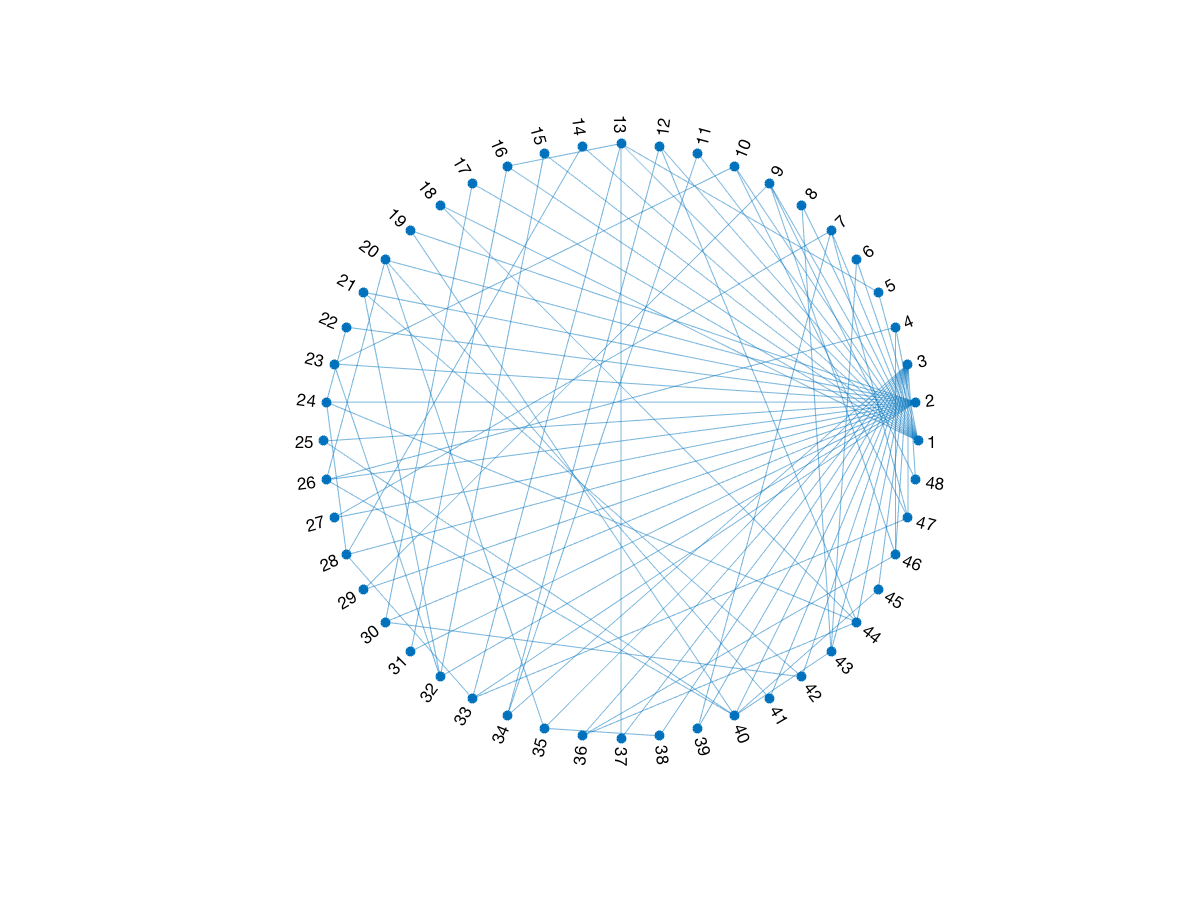
\includegraphics[width=6cm]{fig/disjoint_graph} 
  &   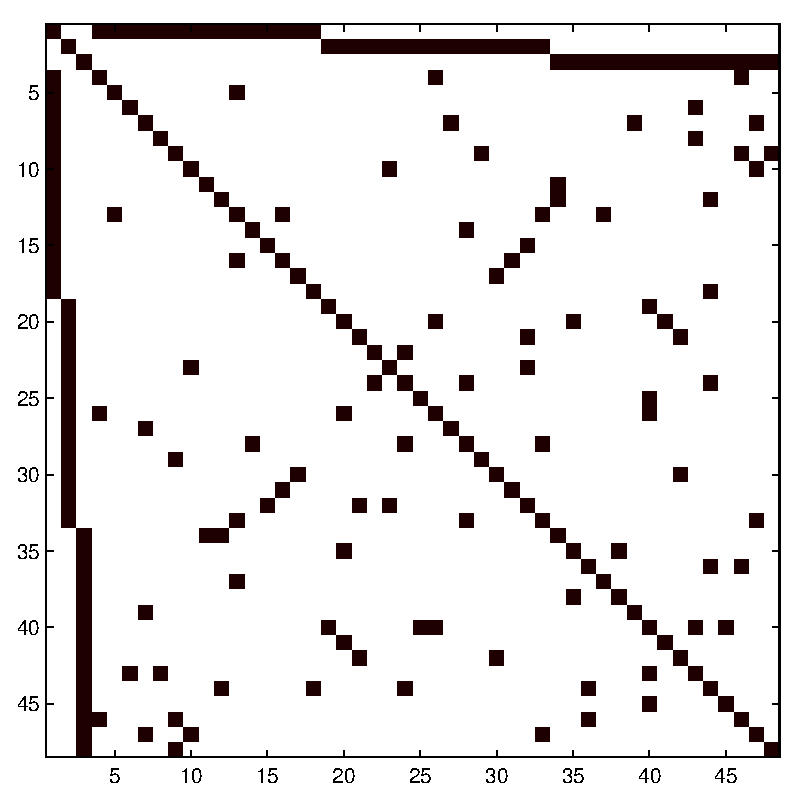
\includegraphics[width=3.5cm]{fig/disjoint_true}
   \\    (a) \textit{model 1} & (b)  structure of concentration matrix for \textit{model 1} \\
      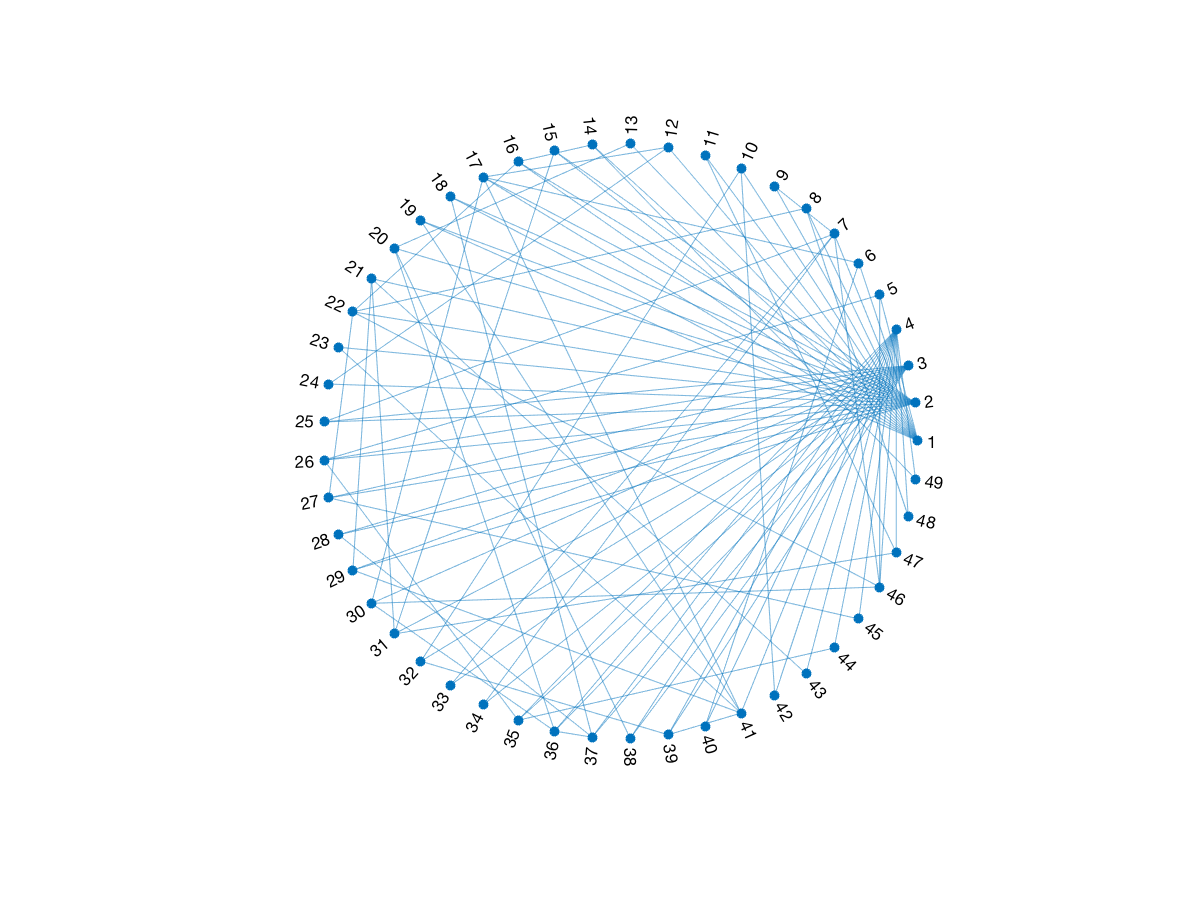
\includegraphics[width=6cm]{fig/over_graph} 
  &   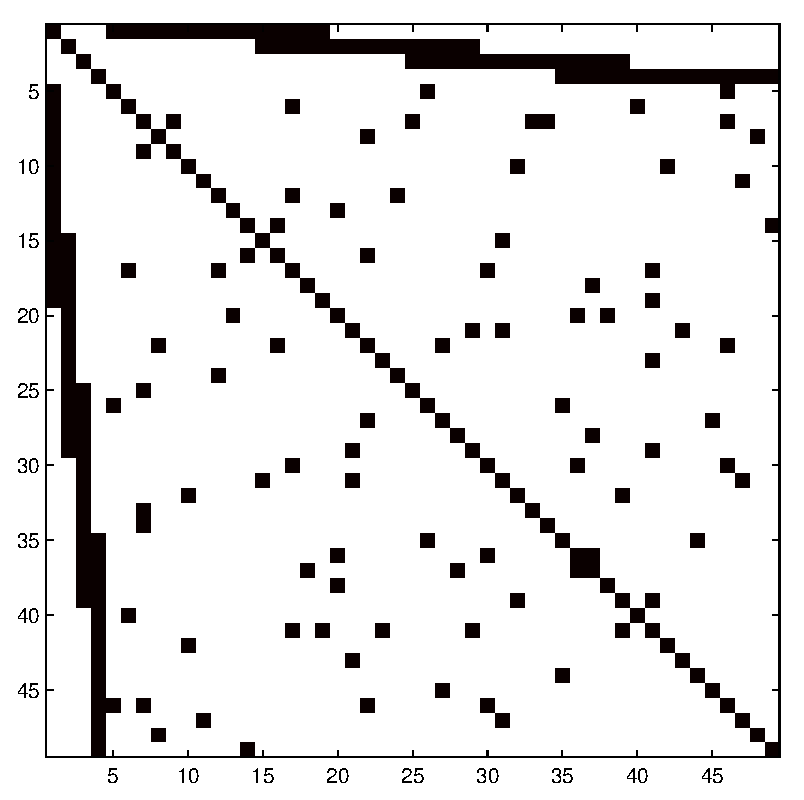
\includegraphics[width=3.5cm]{fig/overlap_true}
   \\    (c) \textit{model 2} & (d)  structure of concentration matrix for \textit{model 2} \\
      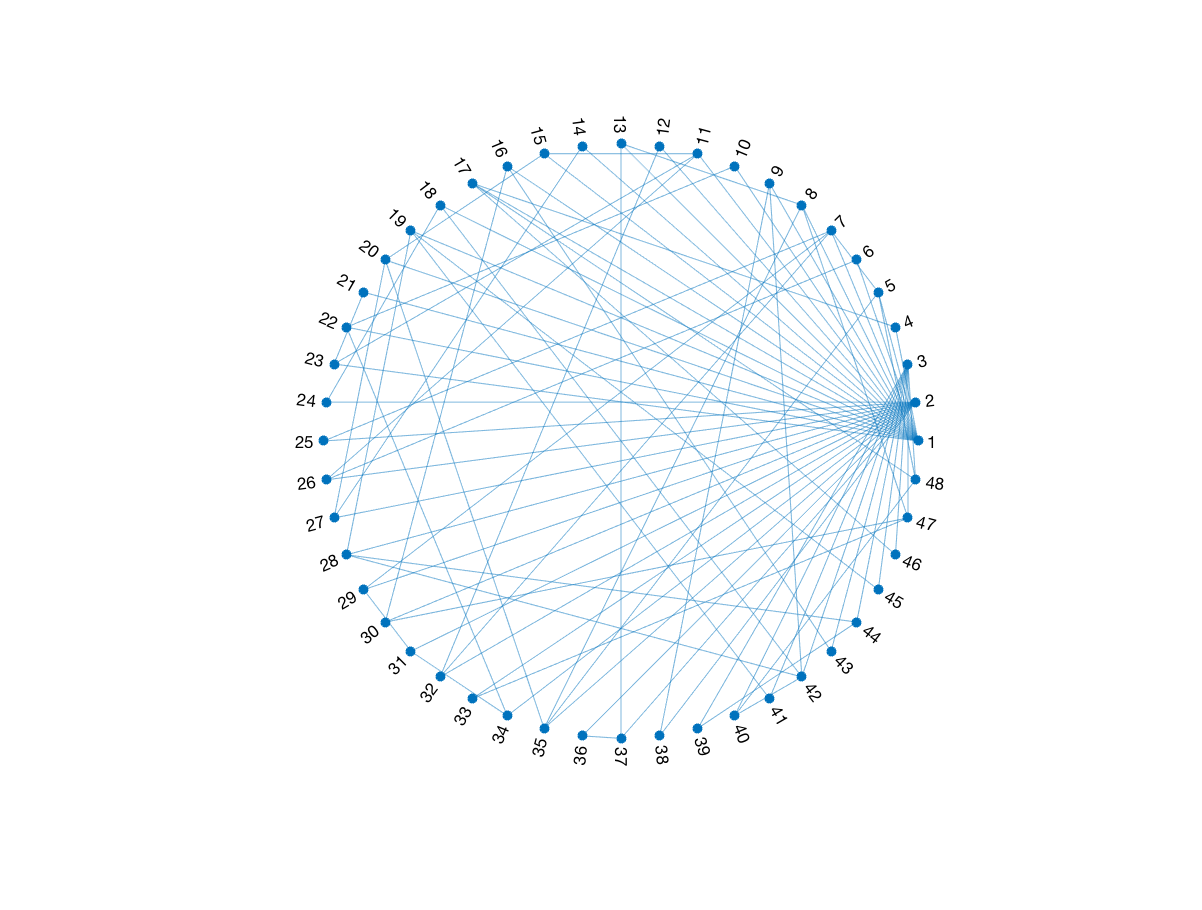
\includegraphics[width=6cm]{fig/diff_graph} 
  &   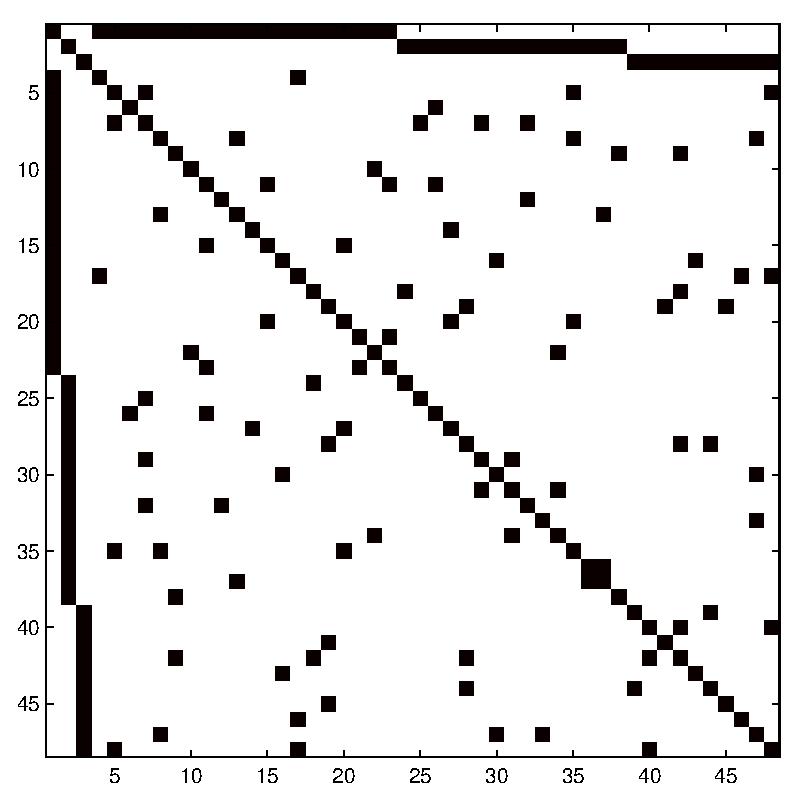
\includegraphics[width=3.5cm]{fig/diff_true}
   \\    (e) \textit{model 3} & (f)  structure of concentration matrix for \textit{model 3}
\end{tabular}
\caption{ Structures of graphical models for the synthetic experiments}
\end{figure}

%The graphs associated to the figures
%\begin{figure}
%\hfill
%\subfigure[\textit{Model 1}]{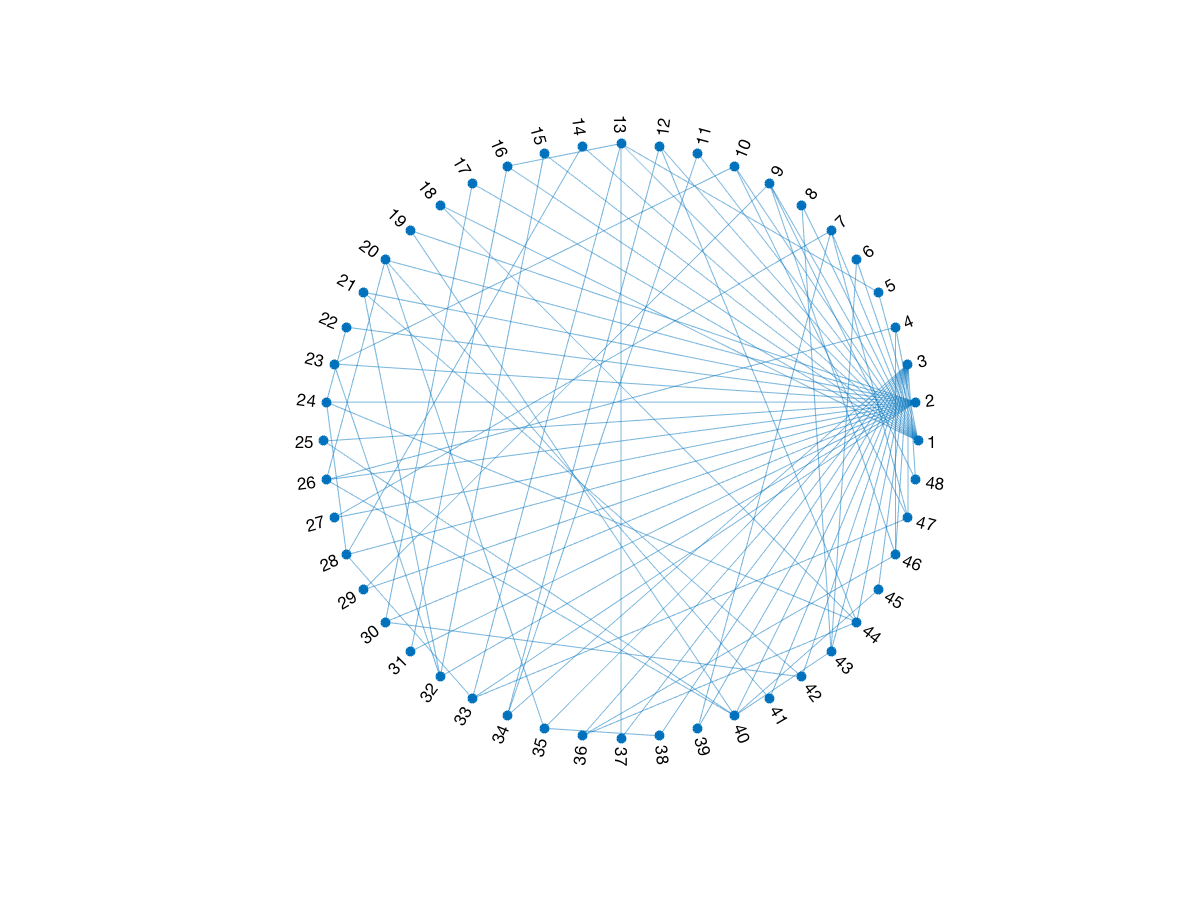
\includegraphics[width=8cm]{fig/disjoint_graph}}
%\hfill
%\\
%\subfigure[\textit{Model 1}]{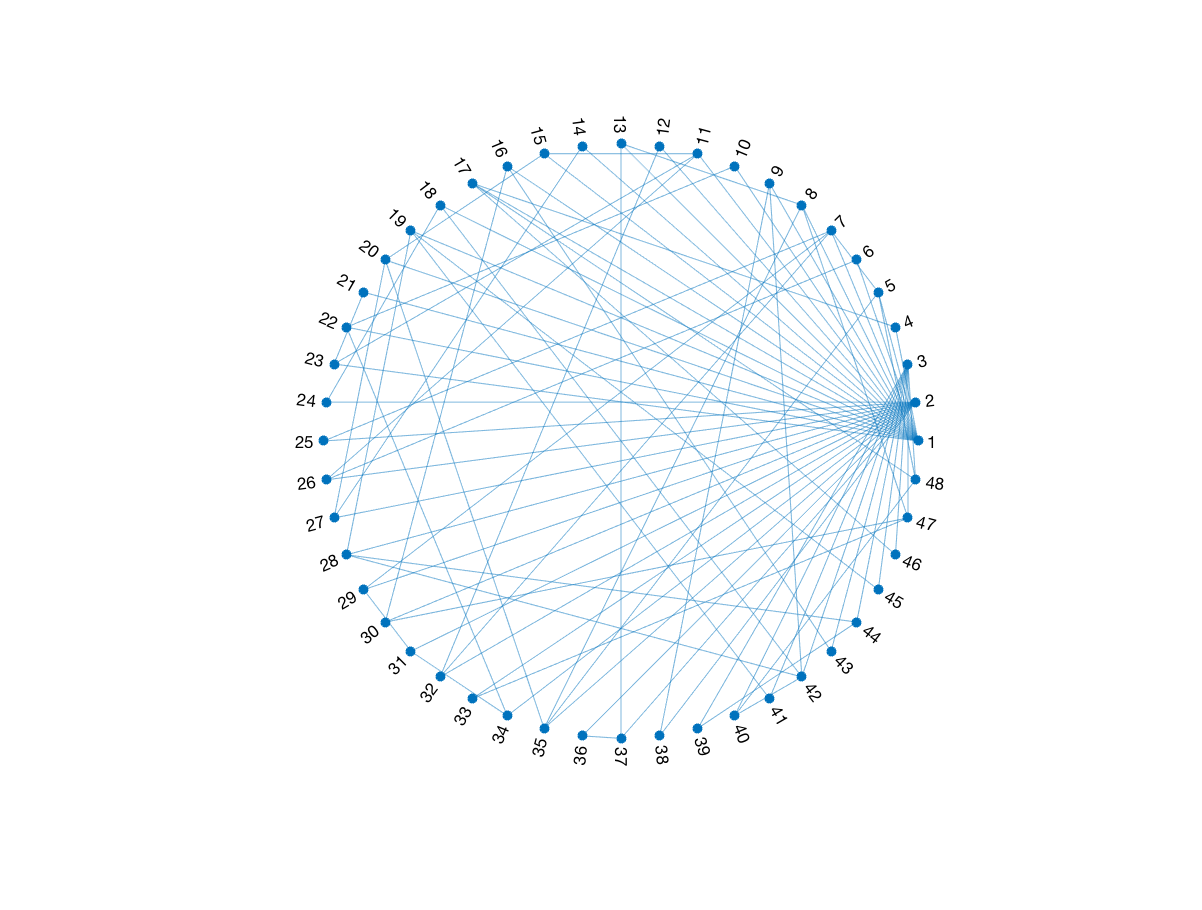
\includegraphics[width=8cm]{fig/diff_graph}}
%\hfill
%\subfigure[\textit{Model 1}]{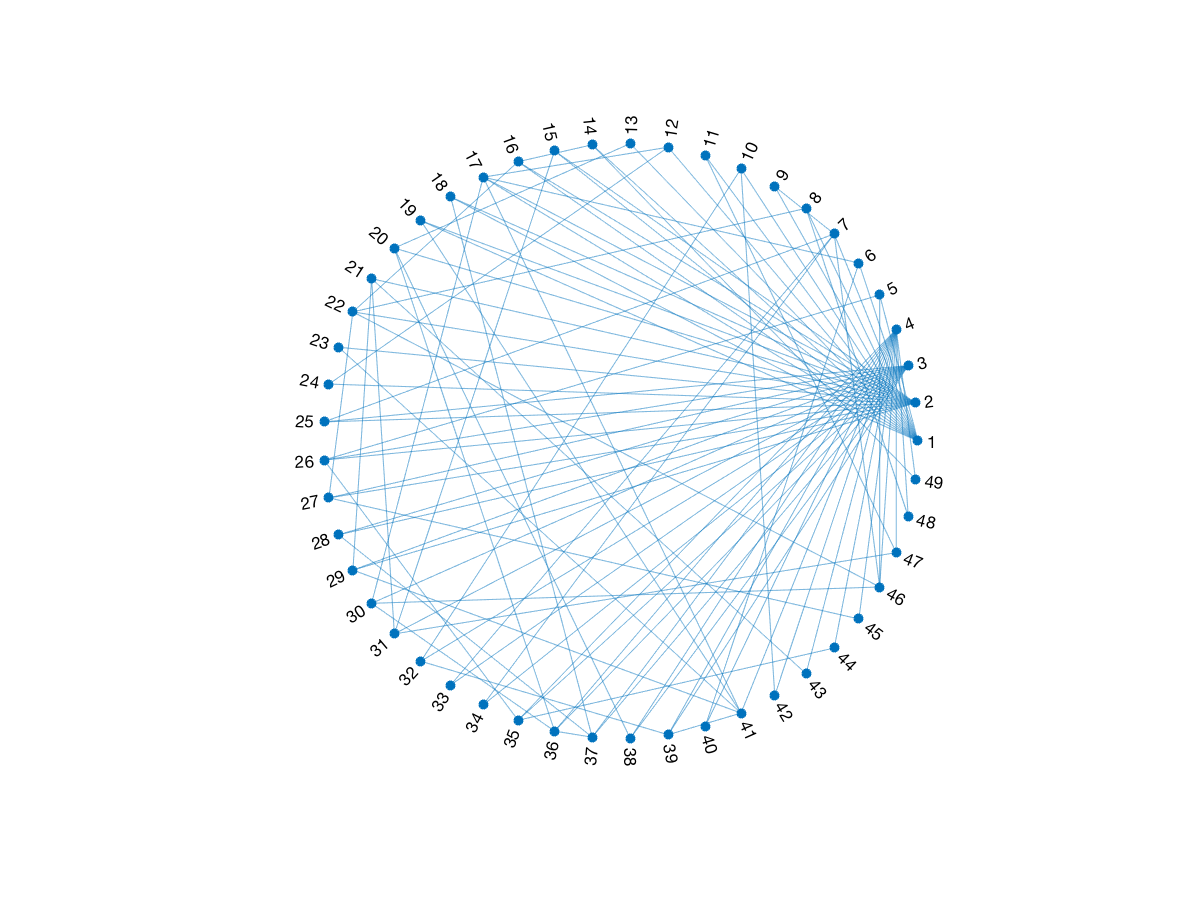
\includegraphics[width=8cm]{fig/over_graph}}
%\caption{Graphical model structures of synthetic experiments}
%\end{figure}

\begin{figure}
\center
\begin{tabular}{cccc}
      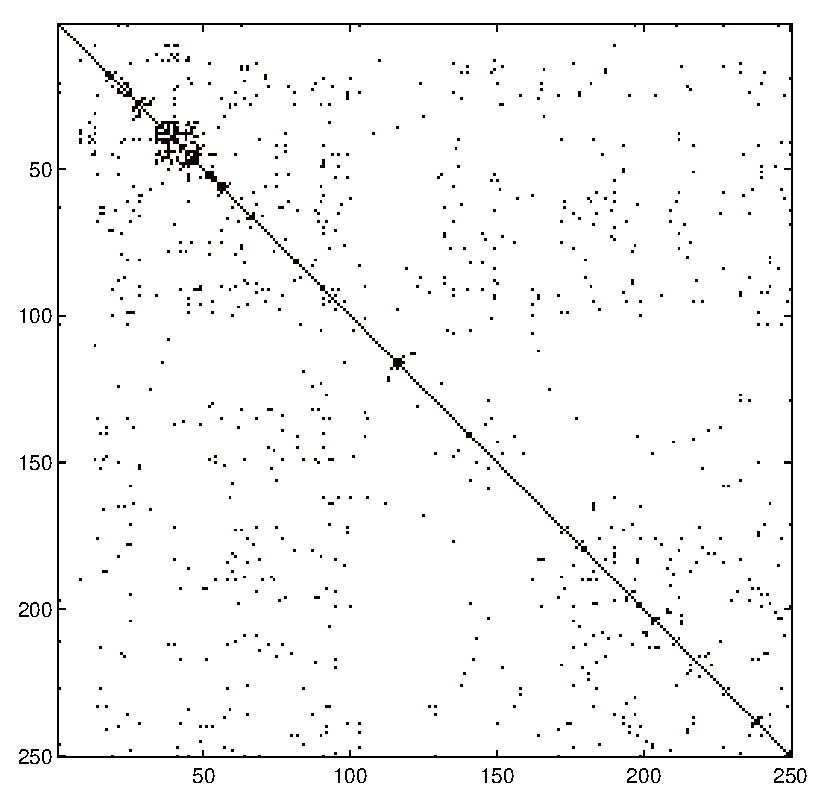
\includegraphics[width=4cm]{fig/MILE_Som}
  &   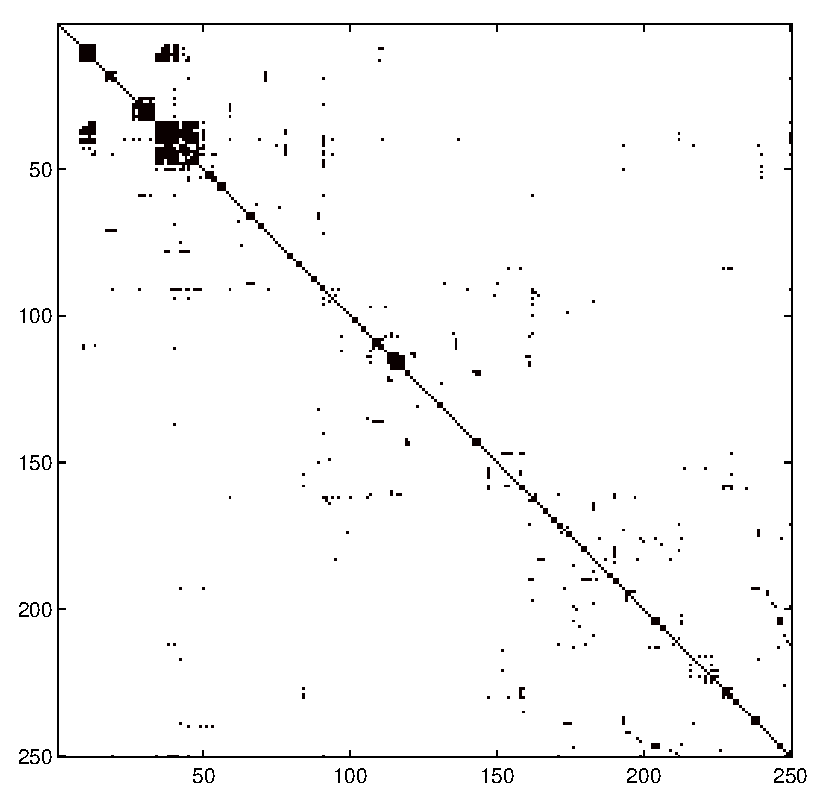
\includegraphics[height=3.8cm]{fig/MILE_Ssl_ordered}
   \\   (a)  $\hat{S}$ $\ell_1+\tr$  & (b) $\hat{S}$ ours 
\end{tabular}
\caption{Sparse component for our method (a) for maximum log-likelihood regularized by $\ell_1+\tr$ (b) }
\end{figure}

\end{document}

%\section*{References}
\bibliographystyle{apalike}
\bibliography{lvggm}